\documentclass{article}
\usepackage[utf8]{inputenc}
\usepackage[margin=1in]{geometry}
\usepackage[sorting=ynt]{biblatex}
\usepackage{graphicx}
\usepackage{subcaption}
\usepackage{authblk}
\graphicspath{{figures/}}
\addbibresource{biblio.bib}

\renewcommand{\baselinestretch}{1.3}
\renewcommand{\abstractname}{\Large Abstract}

\title{Faster Clustering Using Non-Backtracking Random Walks}
\author{Brian Rappaport, Anuththari Gamage, Shuchin Aeron}
\affil{Tufts University}
\date{}

\begin{document}
\maketitle

\begin{abstract}

\end{abstract}


\section{Introduction}

Clustering or classification is traditionally one of the main machine learning tasks, with applications practically everywhere one would want to use machine learning. We consider clustering as a set of elements, using the existence or strength of pairwise interactions between elements as the edges of a graph. 

In this project we will explore efficient and reliable ways of clustering nodes into groups/communities based on pairwise (noisy with missing links) interactions (modeled as edges on a graph). Recently in \cite{DSD} the authors propose to impose a metric on the nodes, referred to as diffusion state distance, or DSD, derived using random walks on the graph to derive a robust affinity measure between nodes followed by spectral clustering \cite{Luxburg}. On the other hand, in another recent paper \cite{NodeEmbed} the authors generate "sentences" of nodes by random walks on the graph as in word2vec \cite{word2vec} followed by embedding the sentences of nodes using a popular method, namely SGNS, for finding Euclidean word embeddings for NLP tasks \cite{LevyGoldberg}.

In the first part of this project we want to numerically explore the connection between these two approaches. While the approach in \cite{DSD} builds upon the limiting DSD, that can be computed in closed form, between nodes it is computationally expensive for large graphs (?? - read the paper). On the other hand the approach in \cite{NodeEmbed} is computationally more attractive it being based on SGNS using SGD like methods that are known to scale well for large problem sizes.

\section{Description}

The Stochastic Block Model is a commonly used graph model for community detection. It builds off of the classical Erdős-Rényi $G(n,p)$ random graph model, wherein each edge of a graph with $n$ nodes is formed with probability $p$. In SBM (technically the planted partition model), $G(n,p)$ is additionally given $k$ clusters, and the probability an edge is formed within the cluster is $a$ while intercluster edges are formed with probability $b$. Clearly, $b$ should be lower than $a$ in order to form an assortive graph. In our work, we have elected to make $b$ proportional to $a$, so $b = \lambda a$ where $\lambda$ is between 0 and 1. Our model is represented as $S(n,k,p,\lambda)$.

[add hubs and spokes model description?]

In order to generate sentences for use in the word2vec stochastic gradient descent algorithm, we need to perform random walks on the graphs. Since the graphs are unweighted, this is simply a matter of choosing at random among the neighbors of each node. We perform a certain number of walks starting from each node to a specific length. Here we also can set the walks to be reluctantly backtracking, where the walk will choose to return to a node immediately after leaving it only if it had no other possible choices. We will also not perform walks on any isolated nodes.

Once the sentences have been formed, we use an existing implementation of word2vec\cite{word2vec}. This takes a corpus of sentences (in this case, the random walks on the graph) and embeds them into $d$-dimensional space by means of stochastic gradient descent. Details on this algorithm can be found in \cite{word2vec}.

\section{Theory}

[section 6 of \cite{Luxburg}, http://www.cs.yale.edu/homes/spielman/561/2012/lect10-12.pdf, Meila and Shi (2001), more...]

\section{Results}

\begin{figure}[h]
 
\begin{subfigure}{0.5\textwidth}
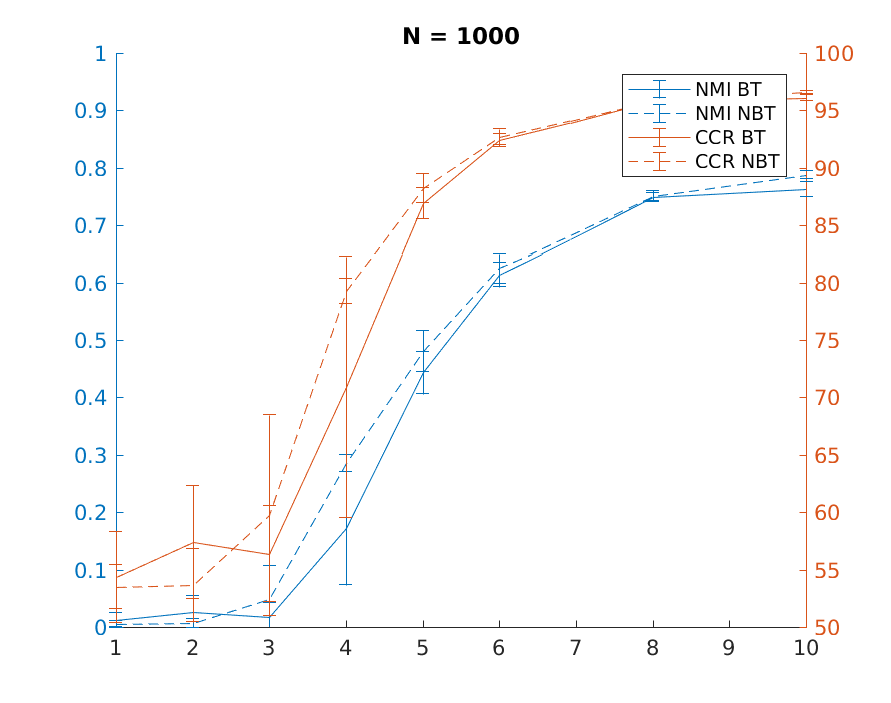
\includegraphics[width=.95\linewidth]{N1000variedc} 
\caption{1000 data points}
\label{fig:subim1}
\end{subfigure}
\begin{subfigure}{0.5\textwidth}
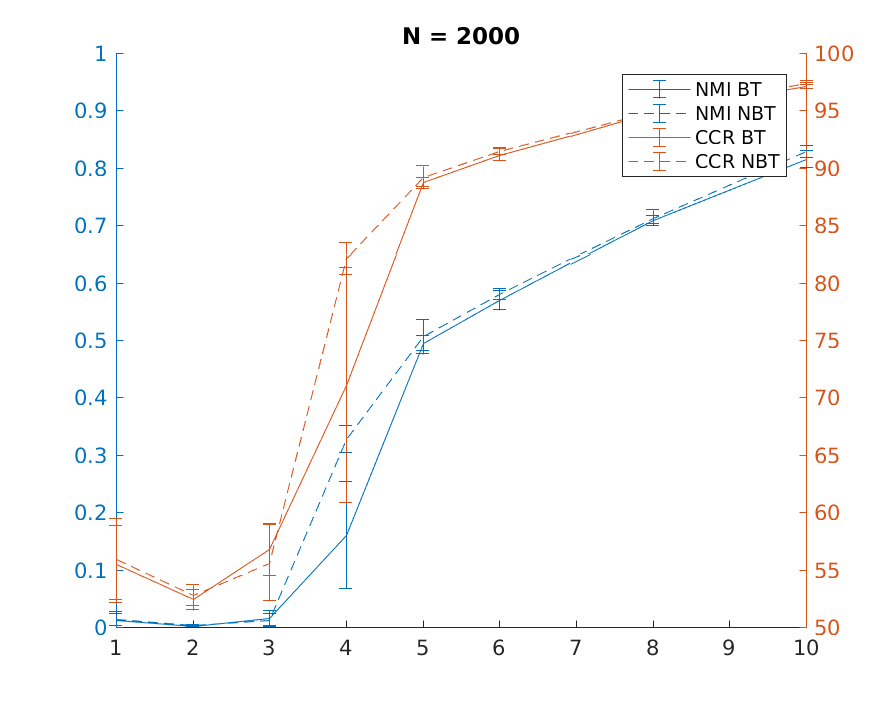
\includegraphics[width=.95\linewidth]{N2000variedc}
\caption{2000 data points}
\label{fig:subim2}
\end{subfigure}
\caption{Accuracy of these algorithms, measured with two different metrics, correct classification rate and normalized mutual information. The x-axis c measures the sparsity of the graph, where an edge is made with probability c/N.}
\label{fig:image2}
\end{figure}

\printbibliography

\end{document}